\section{The ping-pong lemma}\label{sec:lemma}

\subsection{Words and free groups}
Fix four letters $S = \{a, a^{-1}, b, b^{-1}\}$, with $(s^{-1})^{-1} = s$. A
word $s_1 s_2 \cdots s_n$ in $S$ is \emph{reduced} if no letter is next to its
inverse, that is, $s_{k+1} \ne s_k^{-1}$ for every $k$. The first letter can be
any of four and each later letter any of three, so there are
$4 \cdot 3^{n-1}$ reduced words of length $n \ge 1$.

The \emph{free group} $F(a,b)$ is the set of reduced words, including the
empty word~$1$. To multiply two of them, write one after the other and cancel
adjacent pairs $s s^{-1}$ until the word is reduced. If $a$ and $b$ are
elements of a group $G$, there is a unique homomorphism
$\varphi \colon F(a,b) \to G$ that sends each letter to the element of the same
name. Its image is the subgroup $\gen{a, b}$.

\begin{definition}\label{def:free}
Elements $a, b$ of a group $G$ \emph{freely generate a free group of rank~$2$}
if $\varphi$ is injective. Equivalently, no nonempty reduced word in $a^{\pm1}$
and $b^{\pm1}$ is equal to $1$ in $G$. Then $\gen{a,b} \cong F(a,b)$.
\end{definition}

The \emph{Cayley graph} of $F(a,b)$ has a vertex for each element $g$ and
edges from $g$ to $ga$ and from $g$ to $gb$. Every vertex has four neighbors,
$ga^{\pm1}$ and $gb^{\pm1}$. The graph is a tree, because a closed path
without backtracking would spell a nonempty reduced word equal to~$1$. The
ball of radius $n$ about $1$ contains
$1 + \sum_{k=1}^{n} 4 \cdot 3^{k-1} = 2 \cdot 3^n - 1$ elements;
see Figure~\ref{fig:tree}.

\begin{figure}[htbp]
  \centering
  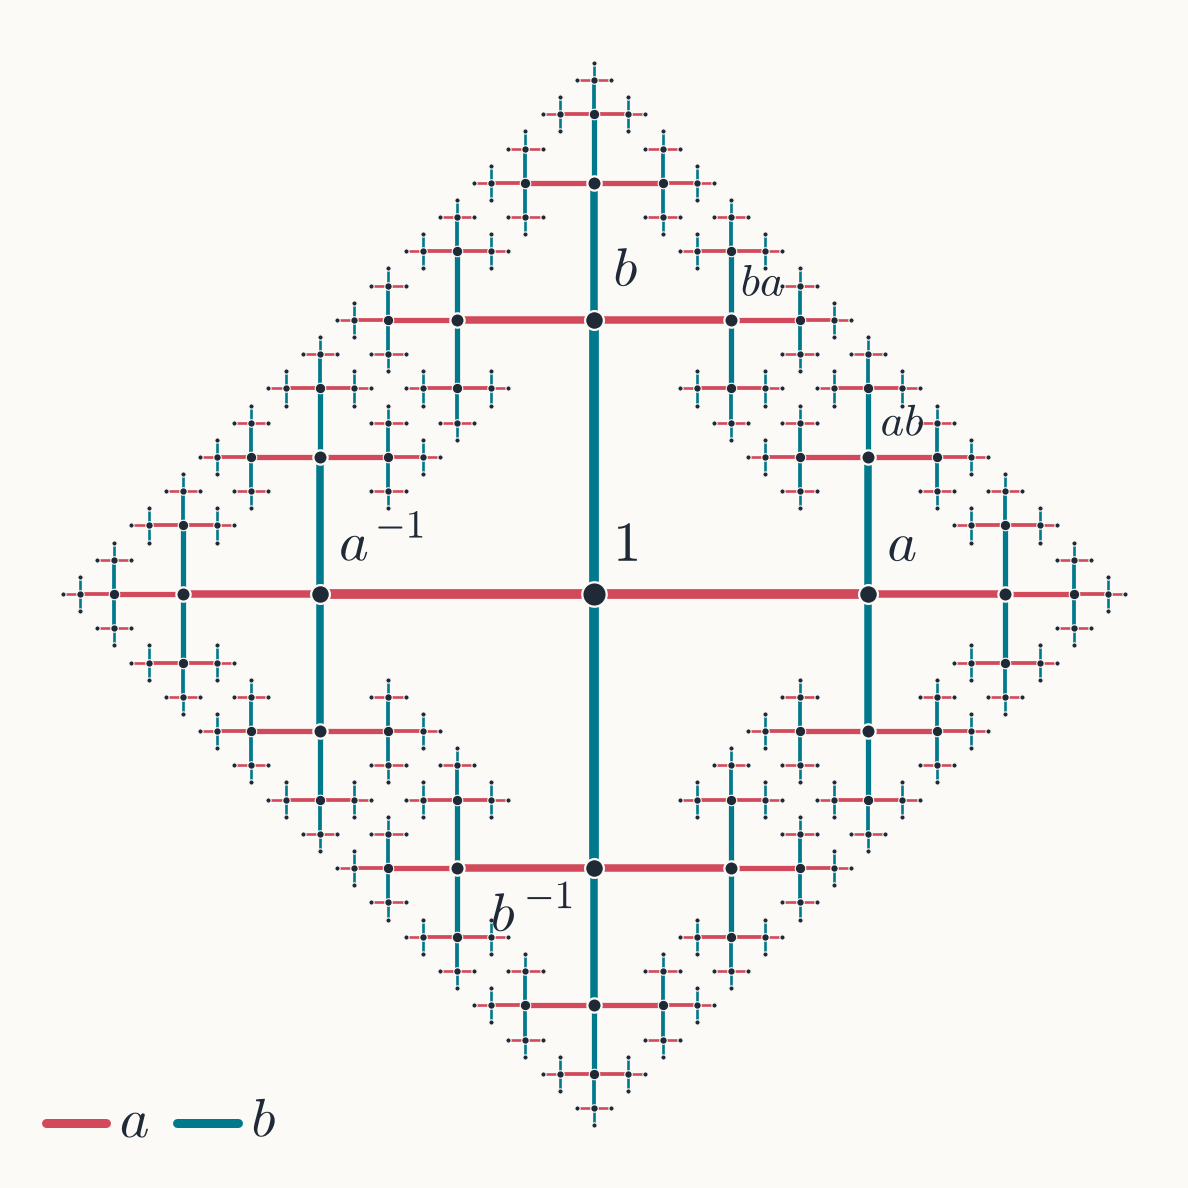
\includegraphics[width=0.40\linewidth]{cayley-tree.png}
  \caption{The Cayley graph of $F(a,b)$ out to distance $5$ from $1$:
  $2 \cdot 3^5 - 1 = 485$ vertices. Edges from $g$ to $ga$ are horizontal
  (red) and edges from $g$ to $gb$ are vertical (teal). Edge lengths halve at
  each step, so the tree fits in the plane.}
  \label{fig:tree}
\end{figure}

\subsection{The four-set form}
Here is the main statement of this project.

\begin{theorem}[Ping-pong lemma]\label{thm:pingpong}
Let a group $G$ act on a set $X$ and let $a, b \in G$. Suppose that
$D_a, D_{a^{-1}}, D_b, D_{b^{-1}} \subseteq X$ are nonempty and pairwise
disjoint, and that
\begin{equation}\label{eq:pingpong}
  s(D_t) \subseteq D_s \qquad \text{for all } s, t \in S \text{ with } t \ne s^{-1}.
\end{equation}
Then $a$ and $b$ freely generate a free group of rank~$2$.
\end{theorem}

In words: each letter $s$ maps three of the four sets, all but $D_{s^{-1}}$,
into its own set $D_s$. Figure~\ref{fig:foursets} shows the hypothesis for $a$
and for~$b$.

\begin{proof}
Let $w = s_1 s_2 \cdots s_n$ be a reduced word with $n \ge 1$. We show that
$w \ne 1$ in $G$. Since $S$ has four letters, we can choose $t \in S$ with
$t \ne s_1$ and $t \ne s_n^{-1}$. Pick $x \in D_t$.

We claim that $s_k s_{k+1} \cdots s_n x \in D_{s_k}$ for $k = n, n-1, \dots, 1$.
For $k = n$ this says $s_n x \in D_{s_n}$, which is \eqref{eq:pingpong} with
$s = s_n$, since $t \ne s_n^{-1}$. If the claim holds for $k+1$, then
$s_k s_{k+1} \cdots s_n x$ lies in $s_k(D_{s_{k+1}})$, which is contained in
$D_{s_k}$ by \eqref{eq:pingpong}, since $s_{k+1} \ne s_k^{-1}$ (the word is
reduced). This proves the claim.

For $k = 1$ the claim says $wx \in D_{s_1}$. Since $t \ne s_1$, the sets
$D_{s_1}$ and $D_t$ are disjoint, so $wx \ne x$. Hence $w$ acts nontrivially
on $X$, and $w \ne 1$ in $G$. Every element of $F(a,b)$ other than $1$ is a
nonempty reduced word, so the kernel of $\varphi$ is trivial.
\end{proof}

\begin{figure}[htbp]
  \centering
  \begin{tikzpicture}[scale=0.82,
      set/.style={draw=#1, fill=#1!16, line width=0.8pt},
      img/.style={draw=#1, fill=#1!50, line width=0.6pt},
      map/.style={-{Stealth[length=2.4mm]}, line width=0.9pt, draw=#1},
      lab/.style={text=ink}]
    % Left: the letter a.
    \begin{scope}
      \draw[set=pa]  ( 1.75, 0) circle (0.95);
      \draw[set=pai] (-1.75, 0) circle (0.95);
      \draw[set=pb]  (0,  1.75) circle (0.95);
      \draw[set=pbi] (0, -1.75) circle (0.95);
      \node[lab] at (2.15, 0.3) {$D_a$};
      \node[lab] at (-1.75, 0) {$D_{a^{-1}}$};
      \node[lab] at (0, 1.75) {$D_b$};
      \node[lab] at (0, -1.75) {$D_{b^{-1}}$};
      \draw[img=pa] (1.20,  0.43) circle (0.21);
      \draw[img=pa] (1.08,  0)    circle (0.12);
      \draw[img=pa] (1.20, -0.43) circle (0.21);
      \draw[map=pa] (0.55, 1.20) to[bend left=12] node[above right=-1pt, text=pa] {$a$} (1.03, 0.58);
      \draw[map=pa] (0.55, -1.20) to[bend right=12] node[below right=-1pt, text=pa] {$a$} (1.03, -0.58);
      \draw[map=pa] (2.30, -0.45) to[out=160, in=-15] (1.21, -0.03);
      \node[text=pa] at (1.95, -0.58) {$a$};
    \end{scope}
    % Right: the letter b.
    \begin{scope}[xshift=7.2cm]
      \draw[set=pa]  ( 1.75, 0) circle (0.95);
      \draw[set=pai] (-1.75, 0) circle (0.95);
      \draw[set=pb]  (0,  1.75) circle (0.95);
      \draw[set=pbi] (0, -1.75) circle (0.95);
      \node[lab] at (1.75, 0) {$D_a$};
      \node[lab] at (-1.75, 0) {$D_{a^{-1}}$};
      \node[lab] at (-0.3, 2.15) {$D_b$};
      \node[lab] at (0, -1.75) {$D_{b^{-1}}$};
      \draw[img=pb] ( 0.43, 1.20) circle (0.21);
      \draw[img=pb] ( 0,    1.08) circle (0.12);
      \draw[img=pb] (-0.43, 1.20) circle (0.21);
      \draw[map=pb] (1.20, 0.55) to[bend right=12] node[above right=-1pt, text=pb] {$b$} (0.58, 1.03);
      \draw[map=pb] (-1.20, 0.55) to[bend left=12] node[above left=-1pt, text=pb] {$b$} (-0.58, 1.03);
      \draw[map=pb] (0.45, 2.30) to[out=-110, in=75] (0.03, 1.21);
      \node[text=pb] at (0.62, 1.88) {$b$};
    \end{scope}
  \end{tikzpicture}
  \caption{The hypothesis \eqref{eq:pingpong} for the letter $a$ (left) and
  the letter $b$ (right). The letter $a$ maps each of $D_a$, $D_b$ and
  $D_{b^{-1}}$ to one of the small dark discs inside $D_a$; nothing is
  required of $a$ on $D_{a^{-1}}$. The pictures for $a^{-1}$ and $b^{-1}$ are
  the mirror images.}
  \label{fig:foursets}
\end{figure}

\begin{remark}\label{rem:variants}
\begin{enumerate}
\item The classical \emph{Schottky hypothesis} is that
$s(X \setminus D_{s^{-1}}) \subseteq D_s$ for every $s \in S$. It implies
\eqref{eq:pingpong}, because $D_t \subseteq X \setminus D_{s^{-1}}$ whenever
$t \ne s^{-1}$. The weaker hypothesis \eqref{eq:pingpong} is the one that
Sanov's example satisfies (Remark~\ref{rem:schottky-fails}).
\item Nothing is special about two generators. For elements
$a_1, \dots, a_k$ with $k \ge 2$ and $2k$ sets $D_{a_i^{\pm1}}$, the same proof
works, since there are $2k \ge 4$ letters to choose $t$ from. For $k = 1$ the
statement is false: if $a = 1$, then $a(D_a) \subseteq D_a$ and
$a^{-1}(D_{a^{-1}}) \subseteq D_{a^{-1}}$ for any two disjoint sets.
\end{enumerate}
\end{remark}

\subsection{The two-set form}
De la Harpe~\cite{delaharpe-2000} proves a version for free products, with two
sets instead of four, and credits the idea to Klein.

\begin{theorem}[Table-tennis lemma]\label{thm:tabletennis}
Let a group $G$ act on a set $X$, and let $H_1, H_2 \le G$ be subgroups with
$\abs{H_1} \ge 3$ and $\abs{H_2} \ge 2$. Let $X_1, X_2 \subseteq X$ be nonempty
and disjoint, with
\[
  h(X_2) \subseteq X_1 \text{ for all } h \in H_1 \setminus \{1\}, \qquad
  h(X_1) \subseteq X_2 \text{ for all } h \in H_2 \setminus \{1\}.
\]
Then the natural map $H_1 * H_2 \to G$ is injective, so
$\gen{H_1, H_2} \cong H_1 * H_2$.
\end{theorem}

\begin{proof}
Every element of $H_1 * H_2$ other than $1$ is a unique alternating product
$w = h_1 h_2 \cdots h_n$ with $n \ge 1$, where each $h_i$ lies in
$H_1 \setminus \{1\}$ or in $H_2 \setminus \{1\}$ and consecutive factors lie
in different subgroups. We show that $w \ne 1$ in $G$, in four cases.

\emph{Case 1: $h_1, h_n \in H_1$.} Pick $x \in X_2$. Then $h_n x \in X_1$,
then $h_{n-1} h_n x \in X_2$, and so on, alternating. Since $h_1 \in H_1$, we
get $wx \in X_1$. As $X_1 \cap X_2 = \emptyset$, $wx \ne x$, so $w \ne 1$.

\emph{Case 2: $h_1, h_n \in H_2$.} Pick $h \in H_1 \setminus \{1\}$. Then
$h w h^{-1} = h h_1 \cdots h_n h^{-1}$ is an alternating product that begins
and ends in $H_1$, so it is not $1$ by Case~1. Hence $w \ne 1$.

\emph{Case 3: $h_1 \in H_1$ and $h_n \in H_2$.} Since $\abs{H_1} \ge 3$, we
can pick $h \in H_1$ with $h \ne 1$ and $h \ne h_1^{-1}$. Then
$h w h^{-1} = (h h_1) h_2 \cdots h_n h^{-1}$, and $h h_1 \ne 1$, so this is an
alternating product that begins and ends in $H_1$. By Case~1 it is not $1$, so
$w \ne 1$.

\emph{Case 4: $h_1 \in H_2$ and $h_n \in H_1$.} Then
$w^{-1} = h_n^{-1} \cdots h_1^{-1}$ is as in Case~3, so $w^{-1} \ne 1$ and
$w \ne 1$.
\end{proof}

\begin{remark}\label{rem:three}
The condition $\abs{H_1} \ge 3$ cannot be dropped. Let $G = \{1, \sigma\}$
act on $X = \{x_1, x_2\}$ by swapping the two points, and let
$H_1 = H_2 = G$, $X_1 = \{x_1\}$, $X_2 = \{x_2\}$. All the other hypotheses
hold, but $\gen{H_1, H_2} = G$ has order $2$, while $H_1 * H_2$ is infinite.
\end{remark}

\begin{example}\label{ex:freeproduct}
If $a$ and $b$ have infinite order, the two-set form with
$H_1 = \gen{a}$ and $H_2 = \gen{b}$ gives $\gen{a,b} \cong \Z * \Z$, a free
group of rank $2$ on $a$ and $b$. Its hypotheses concern all nonzero powers of
$a$ and $b$, but only two sets. For a free product that is not free, let
$\PSL_2(\Z)$ act on the irrational numbers by M\"obius transformations, and let
$s(x) = -1/x$ and $r(x) = 1/(1-x)$. Then $s$ has order $2$ and $r$ has
order $3$ (indeed $r^2(x) = (x-1)/x$). Let $X_1$ be the positive and $X_2$
the negative irrationals. If $x < 0$, then $r(x) \in (0,1)$ and
$r^2(x) = 1 - 1/x > 1$, so $r^{\pm1}(X_2) \subseteq X_1$, and clearly
$s(X_1) \subseteq X_2$. Theorem~\ref{thm:tabletennis} gives
$\gen{r, s} \cong \Z/3 * \Z/2$. Since $s r (x) = x - 1$, the group $\gen{r,s}$
contains $x \mapsto x + 1$ and $x \mapsto -1/x$. These two maps are well
known to generate $\PSL_2(\Z)$, so $\PSL_2(\Z) \cong \Z/3 * \Z/2$.
\end{example}
